\documentclass[tikz,border=4mm]{standalone}
      \usepackage{tikz}
      \usetikzlibrary{arrows.meta,positioning,calc,shapes.geometric}
      \begin{document}
      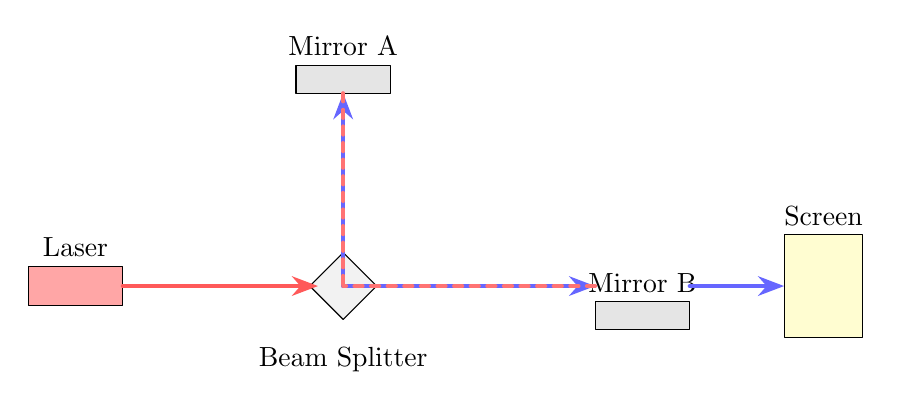
\begin{tikzpicture}[>=Stealth, line cap=round, line join=round]

\draw[fill=red!35] (1.0,4.3) rectangle (2.2,4.8);
\node[above] at (1.6,4.8) {Laser};
\draw[fill=gray!10, rotate around={45:(5,4.55)}] (4.7,4.25) rectangle (5.3,4.85);
\node[below] at (5,3.9) {Beam Splitter};
\draw[->, line width=0.05cm, red!65] (2.2,4.55) -- (4.68,4.55);
\draw[->, line width=0.05cm, blue!60] (5,4.55) -- (5,7.0);
\draw[->, line width=0.05cm, blue!60] (5,4.55) -- (8.2,4.55);
\draw[fill=gray!20] (4.4,7.0) rectangle (5.6,7.35);
\draw[fill=gray!20] (8.2,4.0) rectangle (9.4,4.35);
\node[above] at (5.0,7.35) {Mirror A};
\node[above] at (8.8,4.35) {Mirror B};
\draw[red!55, dashed, line width=0.05cm] (5,7.0) -- (5,4.55);
\draw[red!55, dashed, line width=0.05cm] (8.2,4.55) -- (5,4.55);
\draw[->, line width=0.05cm, blue!60] (9.4,4.55) -- (10.6,4.55);
\draw[fill=yellow!18] (10.6,3.9) rectangle (11.6,5.2);
\node[above] at (11.1,5.2) {Screen};

      \end{tikzpicture}
      \end{document}
